% MSRI - SGS Sparsity week 1, Thursday, 2 lecture, 2x 60 minutes

\documentclass{beamer}

\usepackage{amsmath,amssymb,amsthm,mathrsfs,amscd,mathtools}
\usepackage{datetime}
\usepackage{csquotes}
\usepackage{hyperref}
\usepackage{graphicx}
\usepackage{tikz,tikz-cd}
\usetikzlibrary{arrows,shapes}

\usetheme{Metropolis}
\metroset{block=fill}




\newcounter{maincounter}
\newcounter{excounter}

\newtheorem{conjecture}{Conjecture}
% \setbeamercolor{block body}{bg=mDarkTeal!15}
% \setbeamercolor{block title}{bg=mDarkTeal,fg=black!2}


\newcounter{maincounter}
\newcounter{excounter}
\numberwithin{maincounter}{chapter}
\numberwithin{equation}{chapter}
\numberwithin{excounter}{chapter}
\renewcommand{\theexcounter}{\thechapter.\Alph{excounter}}
\newtheorem{lemma}[maincounter]{Lemma}
\newtheorem{proposition}[maincounter]{Proposition}
\newtheorem{corollary}[maincounter]{Corollary}
\newtheorem{remark}[maincounter]{Remark}
\newtheorem{theorem}[maincounter]{Theorem}
\newtheorem{exercise}[excounter]{Exercise}
\newtheorem{example}[maincounter]{Example}

\newtheorem*{crucial}{Crucial Observation}

\newtheorem{conjecture}[maincounter]{Conjecture}
\newtheorem{definition}[maincounter]{Definition}

\def\AA{\mathbb{A}}
\def\BB{\mathbb{B}}
\def\EE{\mathbb{E}}
\def\HH{\mathbb{H}}
\def\DD{\mathbb{D}}
\def\NN{\mathbb{N}}
\def\RR{\mathbb{R}}
\def\TT{\mathbb{T}}
\def\CC{\mathbb{C}}
\def\ZZ{\mathbb{Z}}
\def\PP{\mathbb{P}}
\def\QQ{\mathbb{Q}}
\def\FF{\mathbb{F}}
\def\GG{\mathbb{G}}
\def\LL{\mathbb{L}}
\def\MM{\mathbb{M}}
\def\SS{\mathbb{S}}
\def\UU{\mathbb{U}}
\def\XX{\mathbb{X}}


%%% Philipp's macros

\newcommand{\dom}[1]{{\mathrm {dom}}({#1})}
\newcommand{\sman}[1]{{#1}^{\mathrm{sm,an}}}
\newcommand{\ansm}[1]{{#1}^{\mathrm{an,sm}}}
\newcommand{\sm}[1]{{#1}^{\mathrm{sm}}}
\newcommand{\anE}{\mathrm{an}}
\newcommand{\an}[1]{{#1}^{\anE}}
\newcommand{\stab}[1]{{\mathrm{Stab}(#1)}}


\newcommand{\hgtexp}{S}

\newcommand{\rank}{{\rm rank}\,}
\newcommand{\Hpoly}[2]{{H^{}_{#1}({#2})}}
\newcommand{\poly}[2]{{#1^{}({#2})}}
\newcommand{\polyt}[2]{{#1^{\sim}({#2})}}
\newcommand{\polytiso}[2]{{#1^{\sim,{\rm iso}}({#2})}}
%\renewcommand{\graph}[1]{\Gamma({#1})}
\newcommand{\atopx}[2]{{\genfrac{}{}{0pt}{}{#1}{#2}}}
\newcommand{\IP}{{\PP}}
\newcommand{\IG}{{\GG}}
\newcommand{\IH}{{\HH}}
\newcommand{\IC}{{\CC}}
\newcommand{\IR}{{\RR}}
\newcommand{\IT}{{\TT}}
\newcommand{\IRan}{{{\RR}_{\rm an}}}
\newcommand{\IRanexp}{{{\RR}_{\rm an,exp}}}
\newcommand{\RRan}{{\IRan}}
\newcommand{\RRanexp}{{\IRanexp}}
\newcommand{\IRalg}{{\RR}_{\rm alg}}
\newcommand{\IQbar}{{\overline{\QQ}}}
\newcommand{\Kbar}{{\overline{K}}}
\newcommand{\IZ}{{\ZZ}}
\newcommand{\IN}{{\NN}}
\newcommand{\IA}{{\AA}}
\newcommand{\IQ}{{\QQ}}
\newcommand{\IQpbar}{{\overline{\QQ}_p}}
\newcommand{\IQp}{{\QQ_p}}
\newcommand{\ts}[1]{{T}_0({#1})}

\newcommand{\cC}{{\mathcal C}}
\newcommand{\cE}{{\mathcal E}}
\newcommand{\cF}{{\mathcal F}}
\newcommand{\cK}{{\mathcal K}}
\newcommand{\cL}{{\mathcal L}}
\newcommand{\cM}{{\mathcal M}}
\newcommand{\cO}{{\mathcal O}}
\newcommand{\cV}{{\mathcal V}}
\newcommand{\cW}{{\mathcal W}}
\newcommand{\cX}{{\mathcal{X}}}
\newcommand{\cY}{{\mathcal Y}}
\newcommand{\cZ}{{\mathcal Z}}



\newcommand{\defZ}{Z}
\newcommand{\defF}{F}
\newcommand{\defW}{W}
\newcommand{\defC}{C}
\newcommand{\defE}{E}
%\newcommand{\deffam}{F}


\newcommand{\re}[1]{{\rm Re}({#1})}
\newcommand{\imS}{{\rm Im}}
\newcommand{\im}[1]{\imS({#1})}
\newcommand{\imageS}{{\rm im}}
\newcommand{\image}[1]{\imageS({#1})}
\newcommand{\volS}{{\rm vol}}
\newcommand{\vol}[1]{\volS({#1})}
\newcommand{\orth}[1]{{#1}^{\bot}}
\newcommand{\mat}[2]{{\rm Mat}_{#1}({#2})}
\newcommand{\ssm}{\setminus}
\newcommand{\ord}[1]{{\rm ord}({#1})}
\newcommand{\opt}[2]{{\rm Opt}_{#2}({#1})}
\newcommand{\Height}[1]{{H}({#1})}
\newcommand{\trdeg}{{\rm trdeg\,}} 
\newcommand{\geo}[1]{\langle {#1}\rangle_{{\rm geo}}}
\newcommand{\defect}{\delta}
\newcommand{\geodef}{{\delta_{\rm geo}}}
\newcommand{\en}[1]{{\rm End}({#1})}
\newcommand{\Hom}[1]{{\rm Hom}({#1})}
\newcommand{\hommaxR}[1]{\text{\rm Hom}({#1})^{*}_{\IR}}
\newcommand{\arith}{\rm arith}
\newcommand{\sgu}[2]{{#1}^{[{#2}]}}
\newcommand{\oa}[1]{{#1}^{\rm oa}}
\newcommand{\codim}{{\rm codim}}
\newcommand{\lgo}{LGO}
\newcommand{\zcl}[1]{{\rm Zcl}({#1})}


\newcommand{\trans}[1]{{#1}^{T}}

\newcommand{\red}[1]{\textcolor{red}{#1}}

\renewcommand{\subset}{\subseteq} %%% Some people think \subset
%%% excludes equality
\renewcommand{\supset}{\supseteq}

\newcommand{\gra}[1]{\mathrm{Gr}({#1})}


\newcommand{\gl}[2]{{\mathrm {GL}}_{#1}({#2})}
\renewcommand{\sp}[2]{{\mathrm {Sp}}_{#1}({#2})}
\newcommand{\autS}{{\mathrm {Aut}}}
\newcommand{\aut}[1]{\autS({#1})}

\newcommand{\spec}[1]{\mathrm{Spec}\,{#1}}

\newcommand{\tor}[1]{{#1}_{\mathrm{tor}}}
\newcommand{\gal}[1]{{\mathrm{Gal}}({#1})}


\newcommand{\zeroset}[1]{\mathscr{Z}({#1})}


\newcommand{\jac}{\mathrm{Jac}}

\newcommand{\bfzeta}{{\boldsymbol{\zeta}}}

\newcommand{\mattt}[4]
{\left(
  \begin{array}{cc}
    {#1} & {#2} \\ {#3} & {#4} 
  \end{array}
\right)}

\newcommand{\matto}[2]
{\left(
  \begin{array}{c}
    {#1} \\ {#2}
  \end{array}
\right)}

\newcommand{\matot}[2]
{\left(
  \begin{array}{cc}
    {#1} & {#2}
  \end{array}
\right)}


\title{MSRI Summer Graduate School \\ Sparsity of Algebraic Points \\
  Day 4: Manin--Mumford and Andr\'e--Oort}
\author{Philipp~Habegger \\ University of Basel \\ \texttt{philipp.habegger@unibas.ch}}
\date{Thursday, June 10, 2021}

\begin{document}

\setlength{\abovecaptionskip}{0pt} 
\setlength{\belowcaptionskip}{0pt} 

\renewcommand{\figurename}{Fig.}


\begin{frame}
  \titlepage
\end{frame}

\section{The Ax--Lindemann--Weierstrass Theorem for Abelian Varieties}


\begin{frame}{A Review of the Abelian Setting}
  Let $A$ be a $g$-dimensional abelian variety defined over $\IC$.
  \begin{itemize}
  \item We can immerse $A$ into some projective space $\IP^n$.

  \item The complex Lie group $A(\IC)$ is a complex torus, \textit{i.e.}, a
    quotient $\IC^g/\Omega$ where $\Omega$ is a discrete subgroup of
    rank $2g$.

  \item The quotient map $u\colon \IC^g\rightarrow \IC^g/\Omega
    =A(\IC)$ can be presented by quasi-periodic holomorphic functions
    $\vartheta_0,\ldots,\vartheta_n \colon \IC^g\rightarrow\IC$.

  \item Fix a basis $(\omega_1,\ldots,\omega_{2g})$ of $\Omega$ and
    define a fundamental domain 
    $$\cF = \{\lambda_1\omega_1+\cdots+\lambda_{2g}\omega_{2g} :
    \lambda_1,\ldots,\lambda_{2g} \in [0,1]\}.$$

    Then all $\vartheta_i|_{\cF}\colon \cF\rightarrow\IC$ are
    definable in $\IRan$.

  \item If $V\subset A$ is an algebraic subset, then the preimage
    $u^{-1}(V(\IC)) \subset\IC^g$ is $\Omega$-periodic.
    The restriction $u|_{\cF}^{-1}(V(\IC))$ is definable in $\IRan$.
  \end{itemize}
\end{frame}

\begin{frame}{Ax--Lindemann Weierstrass for Abelian Varieties}
  \begin{definition}
    Let $A$ be an abelian variety. A \alert{coset} of $A$ is the translate of an
    abelian subvariety of $A$. 
  \end{definition}

  \begin{theorem}[Ax--Lindemann--Weierstrass for abelian varieties]
    Let $C\subset\IC^g$ be a real semi-algebraic curve. After replacing
    $C$ by a non-empty open subset, the Zariski
    closure of $u(C)$ in $A$ is a coset of $A$.
  \end{theorem}

  Historical remark: This theorem follows from Ax's Theorem, the
  functional version of Schanuel's Conjecture. 
  
  Pila--Zannier gave a new proof. Later developments by Bakker, Gao, Klingler,
  Orr, Mok, Pila,
  Tsimerman, Ullmo, and Yafaev.
\end{frame}


\begin{frame}{Step 1: Complexifying the real semi-algebraic $C$}
  
  Let $z_1,\ldots,z_g$ be the complex coordinates of $\IC^g$ with real
  parts $x_1,\ldots,x_g$ and imaginary parts $y_1,\ldots,y_g$. 
  After shrinking $C$ we may assume it is homeomorphic to
  $(0,1)$ and analytic (use Cell Decomposition).

  We consider $x_1|_{C},\ldots,{x_g}|_C,{y_1}|_C,\ldots
  y_g|_{C}$ as restricted coordinate functions.
  Then
  $\mathrm{trdeg}\,\IR({x_1}|_C,\ldots,{y_g}|_C)/\IR=1\Rightarrow
  \mathrm{trdeg}\,\IC({z_1}|_C,\ldots,{z_g}|_C)/\IC=1$.

  Therefore, $C$
  lies in an irreducible complex algebraic curve $C_{\IC}\subset\IC^g$. 

  Let $V$ denote the Zariski closure of $u(C_\IC)$ in $A$. Let $Z$
  denote a maximal irreducible algebraic subset of $\IC^g$ that contains $C_{\IC}$
  and such that $Z(\IC)\subset u^{-1}(V(\IC))$. 
\end{frame}

\begin{frame}{Step 2: Applying the Pila--Wilkie Theorem}


  We do an $\IR$-linear change of coordinates and
  replace $\IC^g$ with $\IR^{2g}$ with the help of our basis of
  $\Omega$. So
  \begin{equation*}
    \IC^g\leadsto \IR^{2g}\quad\text{and}\quad
    \Omega \leadsto \IZ^{2g} \quad\text{and}\quad \cF \leadsto
    [0,1]^{2g}.
  \end{equation*}  

  We continue to use $u$ to denote the uniformization $\IR^{2g}
  \rightarrow A(\IC)$.
  
  The set
  \begin{alignat*}1  
    X =  \{x \in\IR^{2g} : & Z\cap (x+[0,1)^{2g}) \subset x+u|_{[0,1)^{2g}}^{-1}(V)\\
    &\color{gray}{\text{and } Z\cap(x+[0,1)^{2g})\text{ contains a
        neighborhood in $Z$}}
    \}
  \end{alignat*}
  is definable in $\IRan$.
   
\end{frame}

\begin{frame}{A Definable Set} 
  \begin{alignat*}1  
    X =  \{x \in\IR^{2g} : & Z\cap (x+[0,1)^{2g}) \subset x+u|_{[0,1)^{2g}}^{-1}(V)\\
    &\color{gray}{\text{and } Z\cap(x+[0,1)^{2g})\text{ contains a
        neighborhood in $Z$}}
    \}
  \end{alignat*}
  
  \begin{lemma}
    $\{\omega\in\IZ^{2g} :    Z\cap (\omega+[0,1)^{2g})\text{
      contains a neighborhood in $Z$}\} \subset X.$
  \end{lemma}
  \begin{proof}
    Let $\omega \in\IZ^{2g}$ be in the set. 
    Say $y\in Z$ with $y\in \omega+[0,1)^{2g}$. Then $y\in
    u^{-1}(V)$, using $u(Z)\subset V$, and hence $y \in \omega+u^{-1}(V)$
    as $u^{-1}(V)$ is $\IZ^{2g}$-periodic. So $y \in
    \omega+u|_{[0,1)^{2g}}^{-1}(V)$.
  \end{proof}  
\end{frame}

\begin{frame}
  Recall:
  $Z$ is a \alert{complex}  affine variety of positive
  dimension. In real coordinates $\IR^{2g}$ it is an \alert{unbounded} set.
  \begin{minipage}{0.5\linewidth}
    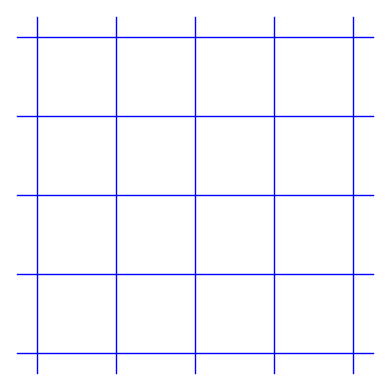
\includegraphics[width=\textwidth]{grid.png}  
  \end{minipage}  \begin{minipage}{0.45\linewidth}
    The set $Z$ meets many translates of the fundamental domain.
    So $X$ contains many integral points $\omega\in\IZ^{2g}$. 

    $H(\omega) = |\omega|_{\mathrm{max}}$
    
    We have $$N(X,T)\gg T$$ as $T\rightarrow\infty$. 
  \end{minipage}
  
  Pila--Wilkie with $\epsilon=1/2$ $\Rightarrow N(X\ssm
  X^{\mathrm{alg}},T)\ll T^{1/2}$

  So $X$ contains a connected, real semi-algebraic curve $R$ passing
  through some $\omega\in\IZ^{2g}$. 
\end{frame}

\begin{frame}
  So $X$ contains a connected, real semi-algebraic curve $R$ passing
  through some $\omega\in\IZ^{2g}$.  $\Rightarrow Z\subset Z-R+\omega$.

  If $x\in R$ then $Z-x\subset u^{-1}(V)$ as
  both sides are complex analytic and since $u^{-1}(V)$ contains a
  non-empty open subset of $Z-x$. Since $u^{-1}(V)$ is
  $\IZ^{2g}$-periodic
  we find $Z-x+\omega\subset u^{-1}(V)$ for all $x\in
  R$. Therefore,
  \begin{equation*}
    Z\subset Z-R_\IC+\omega \subset u^{-1}(V).
  \end{equation*}

  Maximality of $Z \Rightarrow Z = Z-R_{\IC}+\omega \Rightarrow
  -R+\omega \subset \mathrm{Stab}\, Z$.

  \begin{definition}
    The \alert{stabilizer}
       of $Z$ is the subgroup
    \begin{equation*}
      \mathrm{Stab}\, Z = \{v\in \IC^g : v+Z=Z\} \subset\IC^g.
    \end{equation*}
  \end{definition}

  \begin{lemma}
    The stabilizer $\mathrm{Stab}\, Z$ contains a real semi-algebraic curve. 
  \end{lemma}
\end{frame}

\begin{frame}{The Stabilizer Downstairs}
  \begin{definition}
    The \alert{stabilizer} of $V\subset A$ is
    \begin{equation*}
      \mathrm{Stab} V = \{P\in A(\IC) : P+V=V\}. 
    \end{equation*}
  \end{definition}


  \begin{lemma}
     $\mathrm{Stab} V$ is an algebraic subgroup of $A$ of
    positive dimension.
  \end{lemma}
  \begin{proof}
    The stabilizer is Zariski closed as
      $\mathrm{Stab} V = \bigcap_{P \in V} (V-P)$.
    
    % Let $z\in Z$ and $g\in \mathrm{Stab}\,Z$ be arbitrary. Then $z+g\subset Z$,
    % so $u(z) \subset V-u(g)$. We find $V\subset V-u(g)$ and hence
    % $u(g)+V=V$ by considering the dimension.
    % It follows that 
    Now use $u(\mathrm{Stab}\,Z) \subset\mathrm{Stab} V$.  
  \end{proof}  
\end{frame}

\begin{frame}{End of the Proof of
    Ax--Lindemann--Weierstrass}

  Recall: $C\subset \IC^g$ is a (suitable) real semi-algebraic curve and $V$ is the
  Zariski closure of $u(C)$ in $A$.

  We know $\dim\mathrm{Stab} V\ge 1$.

  We want to show: $V$ is a coset in $A$. 

  If $\dim V = \dim \mathrm{Stab} V$, then $V$ is a coset and we are
  done.

  Otherwise $1\le \dim \mathrm{Stab} V \le \dim V-1$.
  
  The connected component $B = \mathrm{Stab}^\circ V$ is an abelian
  subvariety of $A$ of positive dimension. Write $q\colon A\rightarrow
  A/B$.

  Project the image $u(C)$ down
  to $A/B$ and use $\dim A/B \le \dim A-1$. This trick allows us to
  conclude the proof by induction on $\dim A$. \qed
\end{frame}

\section{Consequences of Ax--Lindemann--Weierstrass}

\begin{frame}{Ueno Locus}
  ALW (Roughly): the image of a real semi-algebraic curve under
  $u\colon \IC^g\rightarrow A(\IC)$ lies Zariski dense in a coset of
  $A$.
  
  \begin{definition}
    Let $V$ be a subvariety of $A$. The \alert{Ueno locus} of $V$ is 
    \begin{equation*}
      V^{\circ} = \bigcup_{\substack{\text{coset $\cK$ of $A$} \\\text{with $\dim
            \cK\ge 1$ and $\cK\subset
            V$}}} \cK(\IC).
    \end{equation*}
  \end{definition}

  In general this is an \alert{infinite} union of Zariski closed
  subsets of $V$. It is 
  remarkable that $V^{\circ}$  turns out to be Zariski closed in $V$.

  \begin{theorem}[ALW, alternative formulation]
    Let $V\subset A$ be an irreducible subvariety and set
    $X = u|_{\cF}^{-1}(V(\IC))$.
    Then $u(X^{\mathrm{alg}}) = V^{\circ}$.
  \end{theorem}

\end{frame}


\begin{frame}
  \begin{definition}
    Let $V$ be an irreducible subvariety of $A$. A coset $\cK$ of $A$ is
    called a \alert{maximal coset} of $V$ if $\cK\subset V$ and if it is
    a maximal coset of $A$ with respect to inclusion that is contained
    in $V$. 
  \end{definition}

  Let $\cK_1,\ldots,\cK_r$ be cosets of $A$ contained in $V$ with
  $$\cK_1\subsetneq \cdots\subsetneq \cK_r.$$
  Then $r-1\le \dim \cK_r\le V$. So
  any coset  of $A$ that is contained in $V$ is contained in a maximal
  coset of $V$.
\end{frame}

\begin{frame}
  Many authors contributed to the study of $V^{\circ}$ and variants, including
  Abramovich, Kawamata, Ochiai, and Ueno.

  % Remarkably, $V^{\circ}$ is a \alert{Zariski closed}
  % subset of $V$. 
  
  \begin{theorem} 
    \begin{enumerate}
    \item [(i)] If $\cK=P+B$ is a \alert{maximal} coset of $V$ with $B\subset
      A$ an abelian subvariety, then $B$ lies in a finite set
      depending only on $V$. 
    \item[(ii)] The Ueno locus $V^{\circ}$ is \alert{Zariski closed} in $V$.
    \item[(iii)] We have $V^{\circ} = V\Longleftrightarrow
      \dim\mathrm{Stab} V\ge
      1$. 
    \end{enumerate}
  \end{theorem}
  \begin{proof}\renewcommand{\qedsymbol}{}
    I only mention the basic principle behind (i):
      $\cK=P+B$ is a maximal
    coset of $V$, then $\deg B$ is bounded from above in function of
    $V$. Then use that an abelian variety has only finitely many
    abelian subvarieties of bounded degree. 
  \end{proof}
\end{frame}

\begin{frame}
  \begin{proof}[Proof continued]
    Part (ii) follows from (i) and a general result in the 
    dimension theory of fibers of morphisms. 
    % If $B$ is a fixed abelian subvariety of $A$ and $q\colon
    % A\rightarrow A/B$ is the quotient morphism, then
    % a result in algebraic geometry states that
    % \begin{equation*}
    %   \{P\in V(\IC) :    \dim_P q|_{V}^{-1}(q(P)) \ge \dim B\}    
    % \end{equation*}
    % is Zariski closed in $V$. Together with (i) we conclude (ii).

    % Finally,
    If $V^{\circ}=V$ then by (ii) there exists a single culprit $B$ with
    $\dim B\ge 1$ and 
    $P+B\subset V$ for all $P\in V(\IC)$. So $B\subset
    \mathrm{Stab} V$ and in particular $\dim \mathrm{Stab}V\ge 1$.
    Conversely, if $\dim \mathrm{Stab} V \ge 1$, then $P+B\subset V$
    for all $P\in V(\IC)$ where $B=\mathrm{Stab}^{\circ} V$. 
  \end{proof}
\end{frame}

\begin{frame}{Hyperbolic Varieties}
  \begin{definition}
    Let $V$ be an irreducible projective variety over $\IC$.
    We call $V$ \alert{hyperbolic} if
    any holomorphic map $\IC \rightarrow V(\IC)$ is
    constant.
    % \item[(ii)] We say $V$ is of \alert{general type} if its
    %   \alert{Kodaira dimension} equals $\dim V$. 
    % \end{enumerate}
  \end{definition}

  \begin{example}
    \begin{enumerate}
    \item [(i)]    The projective line $\IP^1$ is \alert{not} hyperbolic. Consider
    $z\mapsto [z:1]$.
    \item[(ii)] An abelian variety $A/\IC$ is \alert{not} hyperbolic.
      Indeed, there are many non-constant
      $\IC\rightarrow \IC^g\rightarrow \IC^g/\Omega =A(\IC)$. 
    \item[(iii)] A smooth projective curve $C$ of genus $g\ge 2$ is
      hyperbolic. Indeed, the universal cover of $C(\IC)$ is the open
      unit disk $\Delta$.
      Any holomorphic map $\IC\rightarrow C(\IC)$ lifts to a
      holomorphic map $\IC\rightarrow\Delta$ which is constant by
      Liouville's Theorem.
    \end{enumerate}
  \end{example}
\end{frame}

\begin{frame}
  \begin{theorem} Let $V$ be an irreducible subvariety of $A$. 
    Then
    $$\text{$V$ is hyperbolic}\Longleftrightarrow
    V^{\circ}=\emptyset. $$
  \end{theorem}

  Hector will tell you about \alert{smooth projective varieties of
    general type} next week.

  If $V$ is a smooth subvariety of an abelian variety, then 
  \begin{alignat*}1
    V \text{ is of general type }&\Leftrightarrow\dim
    \mathrm{Stab}(V)=0 \\
    &\Leftrightarrow
    \text{$V^{\circ}$ is
      not Zariski dense in $V$.}
  \end{alignat*}
\end{frame}

\section{The Manin--Mumford Conjecture}

\begin{frame}{Manin--Mumford Conjecture}
  Let $A$ be an abelian variety defined over $\IC$.
  
  \begin{definition}
    The subgroup of points of finite order in $A(\IC)$ is
    $A_{\mathrm{tors}}$.
    
    A \alert{torsion coset} $K$ of $A$
    is
    $$ T+B $$
    with $B$ an abelian subvariety of $A$ and $T\in\mathrm{A}_{\mathrm{tors}}$. 
  \end{definition}

  \begin{theorem}

  Suppose $K\subset\IC$ is a number field and $A$ is an abelian
  variety defined over $K$. 
  Let $V\subset A$ be an irreducible closed subvariety, also defined over a
  number field $K$. Then
  \begin{equation*}
    V(\IC) \cap A_{\mathrm{tors}} \text{ lies Zariski dense in
      $V$}\Leftrightarrow 
    \text{$V$ is a torsion coset of $A$.}
  \end{equation*}
\end{theorem}
\end{frame}

%\section{Arithmetic of Torsion Points}

\begin{frame}{Group-theoretic Properties of Torsion Points} 
  We collect some facts about the torsion points of an
  abelian variety $A\subset\IP^n$ defined over a number field
  $K\subset \IC$.

  As groups we have $A(\IC) \cong \IR^{2g}/\IZ^{2g}$ with $g=\dim A$.

  For $N\in\IZ$ let $A[N] = \ker \text{(multiplication-by-$N$)}
  \subset A(\overline K)$.
  Then
  \begin{equation*}
    A_{\mathrm{tors}} = \bigcup_{N\ge 1} A[N]
  \end{equation*}
  \begin{lemma}
    $A[N] \cong (\IZ/N\IZ)^{2g}$ if $N\ge 1$.  
  \end{lemma}
\end{frame}


\begin{frame}{The Galois Action}
  Let
  $P=[x_0:\cdots:x_n]\in \IP^n(\overline{K})$ with  $(x_0,\ldots,x_n) \in
  \overline{K}^{n+1}\ssm\{0\}$.
  Say $\sigma\in \absgalk$, then
  \begin{equation*}
    \sigma(P)=  \sigma([x_0:\cdots:x_n]) = [\sigma(x_0):\cdots:\sigma(x_m)]
  \end{equation*}
  is a well-defined action of $\absgalk$ on $\IP^n(\overline K)$.

  If $P\in \IP^n(K)$ we may assume $\forall i:x_i\in K$. So
  $\sigma(P)=P$ for all $\sigma$.
  Conversely, 
  $P\in \IP^n(\overline K)$ with $\sigma(P)=P$ for all $\sigma$ implies
  $P\in \IP^n(K)$.

  \begin{definition}
    Let $P\in \IP^n(\overline K)$. 
    We set $K(P)$ to be the fixed field of the stabilizer
    $\{\sigma\in \absgalk : \sigma(P)=P\}$. 
  \end{definition}


  \begin{equation*}
    \Rightarrow [K(P):K]  = \#\{\sigma(P) : \sigma\in\absgalk \}. 
  \end{equation*}

  We call $\{\sigma(P) : \sigma\in \absgalk\}$ the \alert{Galois
    orbit} of $P$. 
\end{frame}

\begin{frame}
  As $A\subset\IP^n$ is defined over $K$, it is the zero set 
  of  homogeneous polynomials $f_1,\ldots,f_m$ with
  coefficients in $K$. Let $P\in A(\overline K)$. 

  $\Rightarrow \forall i: f_i(P) = 0 
  \Rightarrow \forall \sigma\in\absgalk \forall i: f_i(\sigma(P))=\sigma(f_i(P))=0$

  So $\sigma(P) \in A(\overline K)$ for all $\sigma\in \absgalk$. 

  For $N\in\IN$ the morphism
  $[N]\colon A\rightarrow A$ is, (Zariski-locally), presented
  by a collection of homogeneous polynomials. 
  $$\Rightarrow \sigma([N](P)) = 
  [N](\sigma(P))\text{ for {all} $P\in A(\overline K)$.}$$
  

  We conclude 
  $\sigma(A[N])\subset A[N]$ and
  $\sigma(A_{\mathrm{tors}}) \subset A_{\mathrm{tors}}$ for all $N$
  and all $\sigma$. 

  \begin{definition}
    The Galois action on $A[N]$ induces a representation
    $\rho_N \colon \absgalk\rightarrow\mathrm{Aut}(A[N]) \cong
    \mathrm{GL}_{2g}(\IZ/N\IZ)$.
  \end{definition}
\end{frame}
\begin{frame}
  
  \begin{lemma}
    \begin{enumerate}
    \item[(i)]
      For all $N\in\IN$, the extension  $K(A[N])/K$ is Galois
      of degree at most $N^{4g^2}$.
    \item[(ii)] If $P\in A[N]$, then $[K(P):K]\le N^{2g}$.
    \end{enumerate}
  \end{lemma}
  \begin{proof}
    \vspace{3cm}
  \end{proof}

  We need a \alert{Large Galois Orbit Lemma} as in the proof of the
  Ihara--Serre--Tate Theorem. 
\end{frame}

\begin{frame}{Intermezzo: Serre's Theorem}
  \begin{theorem}[Serre]
    Let $E$ be  an elliptic curve defined over a number $K$
    \alert{without} complex multiplication.
    There exists $c(E)>0$ such that
    if $p\ge c(E)$ is prime number, then $\rho_p \colon
    \absgalk\rightarrow \mathrm{Aut}(E[p]) \cong \mathrm{GL}_2(\IF_p)$
    is surjective.  
  \end{theorem}

  In contrast to the multiplicative setting:
  \begin{itemize}
  \item 
    $K(A[N])/K$ is usually \alert{not} an  \alert{abelian} Galois extension
  \item 
     $K(A(P))/K$ is usually  \alert{not}  even Galois if $P$ has finite
     order. If  $E$
     and $p$ are as in Serre's Theorem and if $P$ has order $p$, then
     \begin{equation*}
       \mathrm{Gal}(\overline K/K(P))=       \rho_p^{-1} \left\{\mattt{1}{*}{0}{*}\right\}
     \end{equation*}
     We have $[K(P):K] = p^2-1 \le p^2$. 
   \end{itemize}   
\end{frame}

\begin{frame}{Masser's Theorem}
  For a root of unity $\zeta$ of order $n$ we have $[\IQ(\zeta):\IQ] =
  \#(\IZ/n\IZ)^\times =\varphi(n)$.
  
  In general there is no ``simple formula'' for the degree of the
  extension $K(A(P))/K$ if $P\in \mathrm{A}_{\mathrm{tors}}$ has order
  $N$.
  Serre's Theorem
  suggests that the degree $[K(P):K]$ of a point of order $N$ grows
  polynomially in terms of $N$ in some cases.

  For a general abelian variety we have Masser's result. 
  
  \begin{theorem}[Masser]
    Let $A$ be an abelian variety defined over a number field $K$. There
    exist $c=c(A)>0$ and $\delta=\delta(A)>0$ with the following
    property. If $P \in A_{\mathrm{tor}}$ has order $N$, then
    $[K(P):K]\ge c N^{\delta}$. 
  \end{theorem}
\end{frame}

\begin{frame}{Proof of the Manin--Mumford Conjecture: Easy Direction}
  Let $A$ be an abelian variety defined over a number field
  $K\subset\IC$.
  Let $V$ be an irreducible subvariety of $A$.

  
  \begin{lemma}
    Suppose $V\subset A$ is a torsion coset. Then $V(\overline K)\cap
    A_{\mathrm{tors}}$ lies Zariski dense in $V$. 
  \end{lemma}
  \begin{proof}
    The torsion points of an abelian variety lie dense with respect to
    the Archmiedean topology and so in particular with respect to the
    Zariski topology. The same holds for torsion cosets. 
  \end{proof}
\end{frame}

\begin{frame}{We have seen this slide before}
  \begin{itemize}
  \item We can immerse $A$ into some projective space $\IP^n$.

  \item The complex Lie group $A(\IC)$ is a complex torus, \textit{i.e.}, a
    quotient $\IC^g/\Omega$ where $\Omega$ is a discrete subgroup of
    rank $2g$.

  \item The quotient map $u\colon \IC^g\rightarrow \IC^g/\Omega
    =A(\IC)$ can be presented by quasi-periodic holomorphic functions
    $\vartheta_0,\ldots,\vartheta_n \colon \IC^g\rightarrow\IC$.

  \item Fix a $\IZ$-basis $(\omega_1,\ldots,\omega_{2g})$ of $\Omega$.
    This is also an $\IR$-basis of $\IC^g$ and allows us to work with
    \alert{real coordinates}, also called \alert{Betti coordinates} $\IR^{2g}$.
    Write $ u\colon \IR^{2g}\rightarrow A(\IC)$, so
    $ u^{-1}(A_{\mathrm{tors}})=\IQ^{2g}$. 

  \item If $V\subset A$ is an algebraic subset, then the preimage
    $ u^{-1}(V(\IC)) \subset\IR^{2g}$ is $\IZ^{2g}$-periodic.
    The restriction $u|_{[0,1)^{2g}}^{-1}(V(\IC))$ is definable in $\IRan$.
  \end{itemize}
\end{frame}

\begin{frame}
  % Let $V\subset A$ be an irreducible subvariety defined over $K$
  % such that $V(\overline K)\cap A_{\mathrm{tors}}$ lies Zariski dense
  % in $V$. 

  \begin{lemma}
    Let $P\in A(\IC)$ be a torsion point of order $N$.
    There exist $x\in \IQ^{2g}$ with $H(x)=N$ and $u(x)=P$. 
  \end{lemma}
  \begin{proof}
    \vspace{2cm}
  \end{proof}
\end{frame}

\begin{frame}
  Recall: The \alert{Ueno locus} $V^{\circ}$  is $\bigcup_{\cK\subset V} \cK$ where $\cK$ is
  a coset of positive dimension. 


  \begin{lemma}
    There exists $N_0(V,A)$ with the following property. If
    $P\in V(\overline K)\cap A_{\mathrm{tors}}$ has order $N$
    and $N\ge N_0(V,A)$, then $P\in V^{\circ}$.
  \end{lemma}
  \begin{proof}\renewcommand{\qedsymbol}{}
    $X =  u^{-1}|_{[0,1)^{2g}}(V(\IC)) \subset \IR^{2g}$
    is definable in $\IRan$.

    Recall $ u(X^{\mathrm{alg}}) = V^{\circ}$ (Ax--Lindemann--Weierstrass).

    \vspace{3cm}

    % Let $\sigma\in \absgalk$. As $V\subset A\subset\IP^n$ is
    % vanishing locus of homogeneous polynomials over $K$, we have $\sigma(P)\in
    % V(\overline K) \Rightarrow P\in V(\overline K)$.

    % Let $P\in V(\overline K) \cap A_{\mathrm{tors}}$ be a point of order
    % $N$, with $N$ large.

    % Say $\sigma\in \absgalk$ then $\sigma(P)\in V(\overline K)$
    % also has order $N$.  The number of
    % Galois conjugates is $[K(P):K]\ge c(A) N^{\delta(A)}$ by
    % Masser's
    % Theorem.
  \end{proof}
\end{frame}

\begin{frame}
  \begin{proof}[Proof continued]
    \vspace{6cm}
% For any $\sigma$, Lemma~\ref{lem:rationalpreimage} provides $x_\sigma
%     \in X\cap\IQ^{2g}$ of height $N$ with $u(x_\sigma) = \sigma(P)$. The
%     number of rational points we obtain in this way is at least
%     \begin{equation}
%       \label{eq:rtlptub}
%       c(N) N^{\delta(A)}. 
%     \end{equation}

%     Now we are ready to apply the Pila--Wilkie Theorem,
%     Theorem~\ref{thm:pilawilkie}. It states
%     \begin{equation}
%       \label{eq:rtlptlb}
%       N(X\ssm X^{\mathrm{alg}},N) \le
%       c(X,\epsilon)N^\epsilon 
%     \end{equation}
%     for all $N\ge 1$, here $c(X,\epsilon)$ depends on $X$ and on $\epsilon
%     > 0$.

%     We set $\epsilon = \delta/2$, which is an invariant that depends only
%     on $A$. We compare (\ref{eq:rtlptub}) and (\ref{eq:rtlptlb}). As we
%     may assume that $N$ is large we must have $x_\sigma \in
%     X^{\mathrm{alg}}$ for some $\sigma\in \absgalk$. 
%     So $\sigma(P) = u(x_\sigma)  \in u(X^{\mathrm{alg}})$.

%     Now we apply Theorem~\ref{thm:imagealg}, a consequence of the
%     Ax--Lindemann--Weierstrass. It follows that $\sigma(P)$ lies in a
%     coset $\sigma(P)+B$ here $B$ is an abelian subvariety of $A$ with
%     $\dim B\ge 1$. As $P$ and also $\sigma(P)$ are torsion points we see
%     that $\sigma(P)+B$ is a torsion coset.
  \end{proof}

\end{frame}

\begin{frame}{Proof of Manin--Mumford}  
  All but finitely many torsion
  points in $A_{\mathrm{tors}}$ have order at least $N(A,V)$.  
  By the last lemma,
  the Ueno locus $V^{\circ}$ lies Zariski dense in $V$.

  But the Ueno locus is always Zariski closed, so 
  $V^{\circ}=V$ and
  $\dim \mathrm{Stab}(V) \ge 1$ from earlier.

  Let $B$ be the connected component of $\mathrm{Stab}(V)^{\circ}$
  containing $0$.
  If $\dim V = \dim B$, then $V$ is a translate of $B$ by a point of
  finite order, we are done.

  Otherwise, the theorem follows by induction on $\dim V$ on
  considering
  $\varphi(V)$ where 
    $\varphi\colon A\rightarrow A/B$ is the quotient morphism. \qed
\end{frame}


\section{Unconditional Andr\'e--Oort for $Y(1)^2$}

\begin{frame}{Recall from Monday}
  \begin{theorem}[Andr\'e--Oort for $Y(1)^2$]
    Let $C\subset Y(1)^2$ be an irreducible curve. Then
    \begin{equation*}
      C \cap Y(1)^2_{\mathrm{special}}\text{ is
        infinite}\quad\Longleftrightarrow\quad \text{$C$ is a special
        curve of $Y(1)^2$}. 
    \end{equation*}  
  \end{theorem}

  Recall also: the set of special points $Y(1)_{\mathrm{special}}$
  is the image under Klein's $j$-function of all $\tau\in\IH$ with
  $[\IQ(\tau):\IQ]$, \textit{e.g.},
  $$\tau = \sqrt{-D}$$
  when $-D\equiv 2,3 \mod 4$. 
  

  We would like to apply the same approach to prove Andr\'e--Oort.

  But $(\mathrm{Re}(\tau),\mathrm{Im}(\tau))$ is
  algebraic but \alert{no longer} rational!   
\end{frame}

\begin{frame}{Pila--Wilkie for Algebraic Points}
  \begin{definition}
    \begin{enumerate}
    \item [(i)] Let $x\in\IC$ be an algebraic number. The
      $\IZ$-minimal polynomial of $x$ is the
      unique polynomial $P=p_dX^d+\cdots+p_0\in \IZ[X]$ that is
      irreducible in $\IQ[X]$ with $p_d\ge
      1,
      \gcd(p_0,\ldots,p_d)=1,$ and $P(x)=0$. The \alert{height} of $x$
      is
      \begin{equation*}
        H(x) = \left(p_d \prod_{z\in \IC : P(z)=0}
          \max\{1,|z|\}\right)^{1/d}\ge 1
      \end{equation*}
      where the product runs over all complex roots of $P$.
    \item[(ii)] Let $(x_1,\ldots,x_m)$ with $x_j$
      algebraic for all $j$. The \alert{height} of
      $(x_1,\ldots,x_m)$ is
      $H(x_1,\ldots,x_m) = \max_{1\le j\le m}H(x_j)$. 
    \end{enumerate}
  \end{definition}
  The exponent $1/d$ is there for normalization purposes. Some authors
  work with $h(x)=\log H(x)$. 
\end{frame}

\begin{frame}
  \begin{itemize}
  \item If $x=p/q$ with $p,q\in\IZ,q\ge 1,\gcd(p,q)=1$, then
    $P=qX-p$ and
    $H(x) = q\max\{1,|p/q|\} = \max\{|p|,q\}.$

    If $m\ge 2$ this bound \alert{differs}  from the one defined
    earlier on rational vectors. The difference is harmless for our purposes.

  \item $H(2^{1/d}) = 2^{1/d}$, just take $P=X^d-2$.

  \item $H(\text{root of unity}) = 1$. Indeed, all roots of the
    $\IZ$-minimal polynomial of a root of unity are on the unit
    circle, moreover, the leading term is $1$.

  \item $H(\sqrt{3}/2) = 2$ as $P = 4X^2-3$ has both roots in
    $[-1,1]$.
  \item Lehmer's polynomial
    $$P=X^{10}+X^9-X^7-X^6-X^5-X^4-X^3+X+1$$
    is
    irreducible and has exactly one root $x=1.1762808\ldots$ outside the
    unit circle. So $H(x)^{10} = x$. Moreover, $x$ is the \alert{smallest known}
    value $>1$ of $H(x)^{[\IQ(x):\IQ]}$. 
    
  \end{itemize}
\end{frame}


\begin{frame}
  Let $x,y\in\IQbar$ and $k\in\IN$. 
  
  The height is Galois invariant:
  $H(\sigma(x))=H(x)$ if $\sigma\in\mathrm{Gal}(\IQbar/\IQ)$.
  
  We have $$H(x^k) = H(x)^k,\text{ }H(x)=H(1/x)
  \text{  (if $x\not=0$),}$$
  $$ H(xy)\le H(x)H(y), \text{ and }H(x+y)\le 2H(x)H(y).$$

  Not all these properties are easy to show with our definition.
  Luckily, there is  an alternative characterization of the height.

  \begin{lemma}
    Let $K$ be a number field and $x\in K$, then
    $$H(x) = \prod_{\substack{v\text{ place} \\\text{of $K$}}}
    \max\{1,|x|_v\}^{[K_v:\IQ_p]/[K:\IQ]}.$$
    Normalization: $|p|_v=1/p$ if $v\mid p$ for a rational prime $p$.
  \end{lemma}
  
\end{frame}

\begin{frame}{Northcott's Theorem}
  Clearly, any root of unity is contained in
  \begin{equation*}
    \{x\in\IQbar : H(x)\le 1\}.
  \end{equation*}
  So a set of algebraic numbers of bounded height need \alert{not} be finite.
  
  We can salvage Northcott's Theorem by 
  bounding \alert{height and  degree}.
  
  \begin{theorem}[Northcott's Theorem]
    Let $d\ge 1$ and $T\ge 1$. The set
    \begin{equation*}
      \{x\in \IC : x \text{ is algebraic with }[\IQ(x):\IQ]\le d\text{
        and }H(x)\le T\}
    \end{equation*}
    is finite. 
  \end{theorem}
\end{frame}


\begin{frame}{The Pila--Wilkie Theorem for Algebraic Points}
  \begin{definition}
    Let $X\subset\IR^m$ be any subset, let $d\ge 1$, and $T\ge 1$. Set
    \begin{equation*}
      N_d (X,T) = \#\{ x\in X\cap \IQbar^m : [\IQ(x):\IQ]\le d
      \text{ and }
      H(x)\le T\}.
    \end{equation*}
  \end{definition}

  Note that $N_d(X,T)<\infty$ for all $T\ge 1$ by Northcott's Theorem. 

  \begin{theorem}[Pila]
    Let $\cS$ be an o-minimal structure, let $d\ge 1$, let $\epsilon
    >0$, and   let $X\subset\IR^m$ be
    definable in $\cS$. 
    There exists  $c(\epsilon,d,X)>0$ such that
    \begin{equation*}
      N_d(X\ssm X^{\mathrm{alg}},T)\le c(\epsilon,d,X) T^\epsilon \quad\text{for
        all}\quad T\ge 1.
    \end{equation*}
  \end{theorem}
\end{frame}

\begin{frame}
  \begin{lemma}
    Let $j(\tau)$ be a special point of $Y(1)$ with $\tau\in\cF$.
    Let $\Delta$ be the discriminant of
    the endomorphism ring of the elliptic curve attached to $j(\tau)$.
    Write $\tau =x+yi$ with
    $x,y\in\IR$, then
    $$[\IQ(x,y):\IQ]\le 4\quad\text{and}\quad H(x,y)\le 16|\Delta|^{5/2}.$$
  \end{lemma}
  \begin{proof}\renewcommand{\qedsymbol}{}
    Set $E = \IC/(\IZ+\tau\IZ)$, then
    $\mathrm{End}(E) = \IZ + \omega \IZ$ where $\omega = f
    \frac{\sqrt{D}+D}{2}$ and $D$ is the discriminant of the field of
    fractions of $\mathrm{End}(E)$ and $f\in\IN$ is its conductor.
    Then $\Delta = f^2D$.
    \begin{equation*}
      \mathrm{Re}(\omega) = f\frac{D}{2} \quad\text{and}\quad
      \mathrm{Im}(\omega) = f\frac{\sqrt{|D|}}{2}
      \quad\text{and}\quad
      |\omega| \le \frac{|\Delta|}{\sqrt{2}}\le|\Delta|
    \end{equation*}
    There exist $a,b,c,d\in\IZ$ with
    $\omega=a+b\tau$ and $\omega\tau = c+d\tau$.
    \begin{equation*}
      \Rightarrow b\tau^2+(a-d)\tau-c=0.
    \end{equation*}
  \end{proof}
\end{frame}

\begin{frame}
  \begin{proof}[Proof continued]       
    So $H(\tau) \le (|b| \max\{1,|\tau|\}^2)^{1/2}$ as $b\not=0$.
    $$\frac{fD}{2}=\mathrm{Re}(\omega) =
    a+b\mathrm{Re}(\tau)\text{ and }\frac{f\sqrt{|D|}}{2}=\mathrm{Im}(\omega)
    = b \mathrm{Im}(\tau).$$
     $\tau$ is in the fundam. domain $\Rightarrow
     |\mathrm{Re}(\tau)|\le \frac 12$ and $|\mathrm{Im}(\tau)|\ge
    \frac{\sqrt{3}}{2}$. So
    \begin{equation*}
      b=|b|\le {f \sqrt{|D|/3}} = \sqrt{|\Delta|/3}
    \end{equation*}
    and
    \begin{equation*}
    |a|\le \frac{b+f|D|}{2} \le \frac{\sqrt{|\Delta|/3} +
        |\Delta|}{2} \le |\Delta|. 
    \end{equation*}
    So
    $\tau = (\omega-a)/b$ and $|\tau|\le
    |\omega-a|\le|\omega|+|a| \le 2|\Delta| $.

    We find $H(\tau) \le (|\Delta|/3)^{1/4} (2|\Delta|)$.
    The estimates for $x=(\tau+\overline\tau)/2$ and $y=(\tau-\overline\tau)/(2i)$ follow from  height
    properties.

    Finally, $\IQ(x,y) =\IQ(\tau,i)$ has degree $\le 4$
    over $\IQ$. 
  \end{proof}
\end{frame}

\begin{frame}{General Approach to Andr\'e--Oort in $Y(1)^2$}
  Let $V\subset Y(1)^2$ be a curve defined over a number field $K$
  that contains infinitely many special points.
  We want to show that $V$ is special.
  
  The set
  \begin{equation}
    \label{def:Xao}
    X = \{(\tau_1,\tau_2) \in \cF^2 : (j(\tau_1),j(\tau_2)) \in V(\IC) \} =
    \boldsymbol{j}|_{\cF^2}^{-1}(V(\IC))
  \end{equation}
  is \alert{definable} in $\IRanexp$. (We identify $\IH$ with
  $\IR\times(0,\infty)$.)

  
  A special point $(z_1,z_2) \in Y(1)^2(\IC)$ is of the form
  $(j(\tau_1),j(\tau_2))$ where  $(z_1,z_2)$ becomes identified with
  $(x_1,y_1,x_2,y_2) \in X$ and
  \begin{equation*}
    [\IQ(x_1,y_1,x_2,y_2):\IQ]\le 16\text{ and }
    H(x_1,y_1,x_2,y_2) \ll \max\{|\Delta_1|,|\Delta_2|\}^3
  \end{equation*}
  here $\Delta_i$ is the discriminant of the endomorphism ring
  of $\IC/(\IZ+\tau_i\IZ)$. 
\end{frame}

\begin{frame}
  \begin{lemma}
    Let $(z_1,z_2)\in V(\IC)$ be special and let $\Delta_i$ denote the discriminant
    of the endomorphism ring of the elliptic curve attached to $z_i$.
    If $\max\{|\Delta_1|,|\Delta_2|\}$ is sufficiently large in terms of
    $V$, then there exists $\sigma\in \absgalk$ with
    $\sigma(z_1,z_2)\in \boldsymbol{j}(X^{\mathrm{alg}})$.   
  \end{lemma}
  
  The proof is as in the Manin--Mumford Theorem, but we need to use
  Pila's version of Pila--Wilkie for algebraic points (of degree $\le
  16$).
  Large Galois orbits are afforded by the \alert{Landau--Siegel}
  Theorem.

  \begin{theorem}[Landau--Siegel]
    For all $\epsilon > 0$ there exists $c(\epsilon)>0$ with
    $$[\IQ(z_1,z_2):\IQ] \ge c(\epsilon)
    \max\{|\Delta_1|,|\Delta_2|\}^{1/2-\epsilon}.$$
  \end{theorem}
\end{frame}

\begin{frame}{Ax--Lindemann--Weierstrass for the $j$-function}
  But what about $\boldsymbol{j}(X^{\mathrm{alg}})$?

  \begin{theorem}[Pila, 2011]
    Let $W\subset\IH^m$ be a connected neighborhood of the
    intersection of an
    irreducible subvariety of $\IC^m$ with $\IH^m$.
    Let $\tau_1,\ldots,\tau_m$ denote the coordinate functions of $\IH^m$.
    Suppose that $j\circ {\tau_1|}_{W},\ldots,j\circ {\tau_m}|_{W}$
    are \alert{not} algebrically independent.
    Then some $j\circ{\tau_k}|_W$ is constant or
  there exist $N\in\IN$ and 
    $k\not=l$ with $\Phi_N(j\circ \tau_k|_W,j\circ \tau_l|_W)=0$ as
    functions on $W$.    
  \end{theorem}
  \vspace{-.2cm}
  
  We take $m=2$ and  $W$ equals $\IH^2$
  intersected with the complexification of a semi-algebraic curve in $X^{\mathrm{alg}}$.
  
  Observe that $j\circ \tau_1|_W$ and $j\circ \tau_2|_W$ are not
  algebraically independent since their image lies in the algebraic curve
  $V\subset Y(1)^2$.
  So one of $j\circ \tau_k|_W$ must be constant or the two coordinates
  are related by a modular transformation polynomial. 
  $\Rightarrow V$ is \alert{special}.  
\end{frame}


\begin{frame}{Conclusion}
  \begin{itemize}
  \item The proof of Manin--Mumford presented using Pila--Wilkie was
    devised by Pila and Zannier.

  \item Pila proved Andr\'e--Oort in $Y(1)^m$ \alert{unconditionally}.
    This approach led to many developments in the last few years. More on
    this tomorrow. 
    
  \item Pila--Wilkie is used \alert{twice} in Pila's proof. Once in a
    \alert{geometric} setting to prove
    Ax--Lindemann--Weierstrass and once in an \alert{arithmetic} setting to count Galois conjugates. 
  \end{itemize}
  
  
\end{frame}

\begin{frame}
  \begin{center}
    Thanks for your attention. The final lecture tomorrow is on unlikely
    intersections. 
  \end{center}
\end{frame}

\end{document}
